\documentclass[letterpaper,12pt]{article}
 \usepackage[utf8]{inputenc}
\usepackage[T1]{fontenc}
% \usepackage[latin9]{inputenc}
\usepackage{amstext}
\usepackage{amsmath}
\usepackage{amssymb}
\usepackage{graphicx}
\usepackage{geometry}
\usepackage{tikz}
\usepackage{esint}
\usepackage{caption}
\usepackage{subcaption}

\geometry{
 letterpaper,
%  total={210mm,297mm},
 left=1.25in,
 right=1.25in,
 top=1.5in,
 bottom=0.5in,
 }
 
 \begin{document}
  \begin{picture}(0,0)
\put(114,-10){
\includegraphics[width=6cm]{Images/un_logo.eps}}
\end{picture}
\begin{center}
\textbf{
 FACULTAD DE INGENIER\'IA\\
 Vicedecanatura Acad\'emica\\
 POSGRADOS \break
  \newline
 PROPOSAL SUBMISSION
}

\end{center}
\vspace{30pt}

% •Título preliminar
% •Justificación
% •Estado del arte
% •Definición del problema
% •Metodología
% •Cronograma aproximado
% •Sectores de impacto de la investigación
% •Referencias bibliográficas 

%checkboxes
\begin{tabular}{l c l c}
 DOCTORAL THESIS: & \framebox[0.5cm][c]{x} & MASTER THESIS: & 
\framebox[0.5cm][c]{}\\
 MASTER FINAL WORK: & \framebox[0.5cm][c]{} & SPECIALIZATION FINAL WORK: & 
\framebox[0.5cm][c]{}\\ 
\end{tabular}
\vspace{20pt}
 \begin{enumerate}
  \item \textbf{BIDDER:} Robinson Andr\'es Jaque Pirab\'an \qquad\qquad 
\textbf{ID:} 80190790
  \item \textbf{PROGRAM:} Phylosophy Doctoral in Computer Science and Systems 
Engineering
  \item \textbf{ADVISOR:} Fabio Augusto Gonz\'alez Osorio\\
  \textbf{DEPARTMENT:} Computer Science and Industrial Engineering
  \item \textbf{TITLE: Kernel Tensor Factorization }%check
  \item \textbf{AREA:} Computer Science
  \item \textbf{LINE OF RESEARCH:} Machine Learning
  \item COMMENTARY WITH ADVISOR APROVAL
  \vspace{120pt}
% % 14. COMENTARIO CON VISTO BUENO DEL DIRECTOR: (calificar los siguientes 
% aspectos: organización, pertinencia, relevancia y originalidad).
  \item BIDDER SIGNATURE 
%  
%  Robinson Andr\'es Jaque Pirab\'an
% % 15. FIRMA DEL PROPONENTE
  \vspace{60pt}
  \item SIGNATURE OF ADVISOR
  \vspace{60pt}
 % 16. FIRMA DEL DIRECTOR (ASESORES)
 % 17. FECHA  
  \end{enumerate}  
  
%   \item \textbf{BACKGROUND AND JUSTIFICATION:}\\
  
% 5. ANTECEDENTES Y JUSTIFICACIÓN: (Indicar los desarrollos previos, 
% circunstancias y condiciones que llevaron a la conclusión de la necesidad y 
% conveniencia del proyecto)

%  \item \textbf{PROBLEM STATEMENT:}\\
% 6. IDENTIFICACIÓN DEL PROBLEMA: 


\clearpage

%Portada

\clearpage

\tableofcontents

\newpage

\section{Basics of tensors}

Tensors are multidimensional arraies. i.e. An $N$-way or $N$-order tensor is an element of tensor product of $N$ vector spaces, each of which has its own coordinate system. A first order tensor is a vector, a second order tensor is a matrix, tensors of higher order are called high-order tensors. The order (ways or modes) of a tensor is the number of dimensions. Figure \ref{fig:3tensor} represents a 3-order tensor $\mathcal{X}\in\mathbb{R}^{I\times J\times K}$.

\begin{figure}[!ht]
\centering
 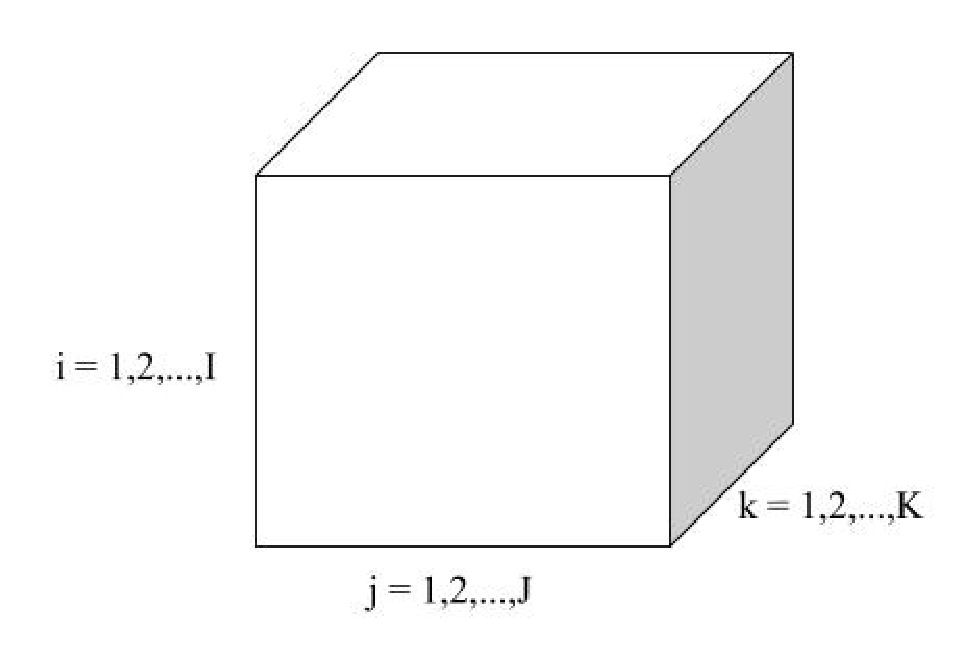
\includegraphics[scale=0.4]{Images/3rd-order_tensor.eps}
 \caption{Third-order tensor}\label{fig:3tensor}
\end{figure}

\textit{Fibers} are defined by fixing every index by one. In a third-order tensor a column is a mode-1 fiber, denoted by $x_{:jk}$; a row is a mode-2 fiber, denoted by $x_{i:k}$; while a tube is a mode-3 fiber, denoted by $x_{i:k}$. \ref{fig:3tensor-fibers} shows a fibers representation in 3rd-order tensor.

\begin{figure}[!ht]
 \centering
 \begin{subfigure}[b]{0.29\textwidth}
  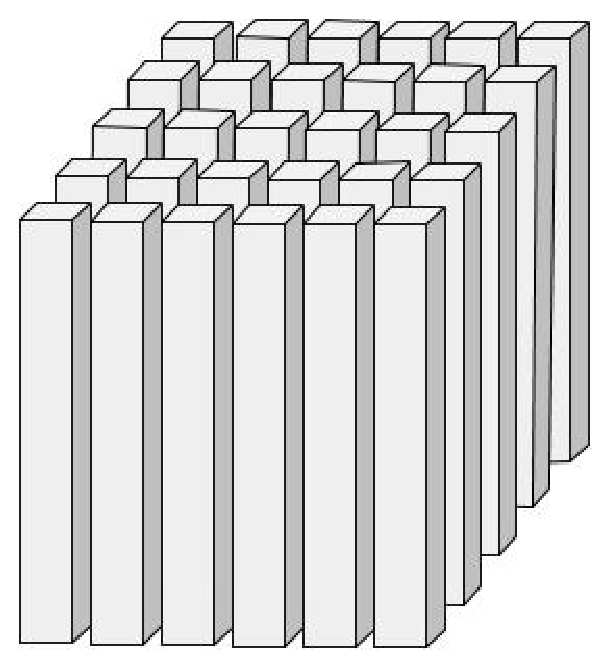
\includegraphics[width=\textwidth]{Images/3rd-order-tensor-fiber_mode-1.eps}
  \caption{columns}\label{fig:3tensor-columns}
 \end{subfigure}
 \begin{subfigure}[b]{0.33\textwidth}
  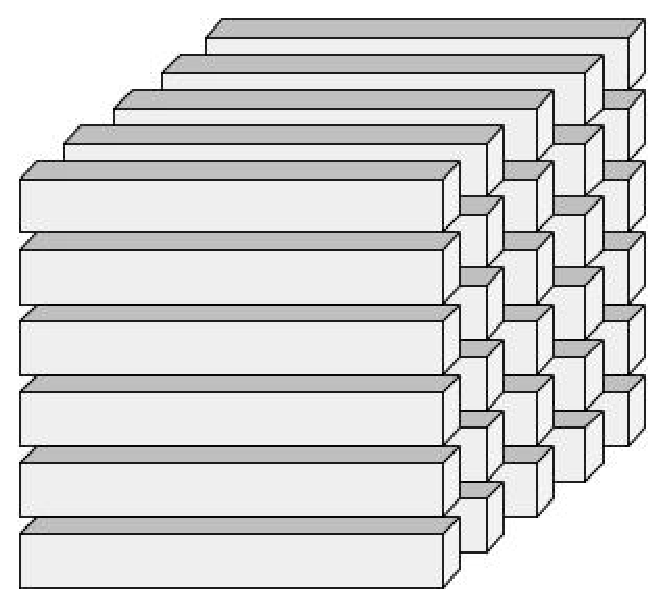
\includegraphics[width=\textwidth]{Images/3rd-order-tensor-fiber_mode-2.eps}
  \caption{rows}\label{fig:3tensor-rows}
 \end{subfigure}
 \begin{subfigure}[b]{0.33\textwidth}
  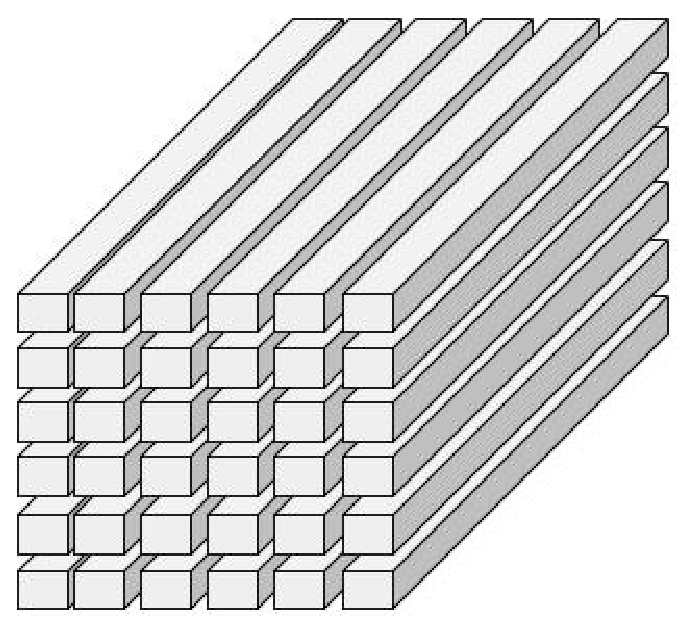
\includegraphics[width=\textwidth]{Images/3rd-order-tensor-fiber_mode-3.eps}
  \caption{tubes}\label{fig:3tensor-tubes}
 \end{subfigure}
\caption{3rd-order tensor fibers}\label{fig:3tensor-fibers}
\end{figure}

\textit{Slices} are two-dimensional sections of a tensor defined by fixing two indexes. For instance, slices of 3rd-order tensor $\mathcal{X}$ are denoted by $X_{i::}$ (horizontal), $X_{:j:}$ (lateral) and $X_{::k}$ (frontal).

%include slices figures when I can

The \textit{norm} of a tensor $\mathcal{X}\in \mathbb{R}^{I_1\times I_2 \ldots \times I_N}$ is analogous to the matrix Frobenius norm, i.e.
\begin{equation}
||\mathcal{X}|| = \sqrt{\sum_{i_1=1}^{I_1}\sum_{i_2=1}^{I_2}\cdots\sum_{i_N=1}^{I_N} x_{i_1i_2\ldots i_N}^2 } 
\end{equation}\label{eq:Frobenius-norm}

%also include here
%inner product of two same-size tensors
% rank one tensors
% simetry
% diagonal tensor

\subsection{Unfolding and Folding Tensors}

\textit{Unfolding} is the process of \textit{matricization} of a tensor. In other words, elements of a tensors are sorted to assemble a matrix. The mode-$k$ unfolding of a tensor $\mathcal{X}\in \mathbb{R}^{I_1\times I_2 \ldots \times I_N}$ is denoted by
 $X_{(k)} \in \mathbb{R}^{I_1\times \prod_{k'\neq k}I_{k'} }$ and arrenges the mode-$k$ tensor fibers as columns of resulting matrix. In addition, Kolda \cite{Kolda2009} presents a more general procedures of unfolding

% figure mode-k unfolding and folding

% \subsubsection{Tensor products}

% \paragraph{Mode-k product}

% \paragraph{Kronecker product}

% \paragraph{Khati-Rao product}

% \paragraph{Hadamar product}

% \paragraph{Outer product}


Ding and Wei \cite{Ding2015} present a fast algorithm for Hankel tensor-vector products.

\cite{Dourbal2016} A method of fast linear transform algorithm synthesis for an arbitrary tensor

\section{Tensor Decomposition}


Tensor decomposition originated with Hitchcock in 1927 \cite{Hitchcock1927}, and the the multi-way model is attribuited to Cattell in 1944 \cite{Cattell1944}.

Tensor works had attention in 60s with Tucker (\cite{Tucker1963}, \cite{Tucker1964}, \cite{Tucker1966}) and Carroll and Chang \cite{Carroll1970} and Harshman in 1970 \cite{Harshman1970} with applications in psychometrics. In 1981 Appellof and Davidson \cite{Appellof1981} used tensor decomposition in chemometrics which have been an popular field of application of tensor decomposition since then.

In last twenty years tensor decomposition applications have expanded to many fields such as signal processing, numberical linear algebra, computer vision, numerical analysis, neuroscience, data mining, graph analysis. Figure \ref{fig:applications} attempt to summarize application fields of tensor decomposition. 

\begin{figure}[!ht]
\centering
 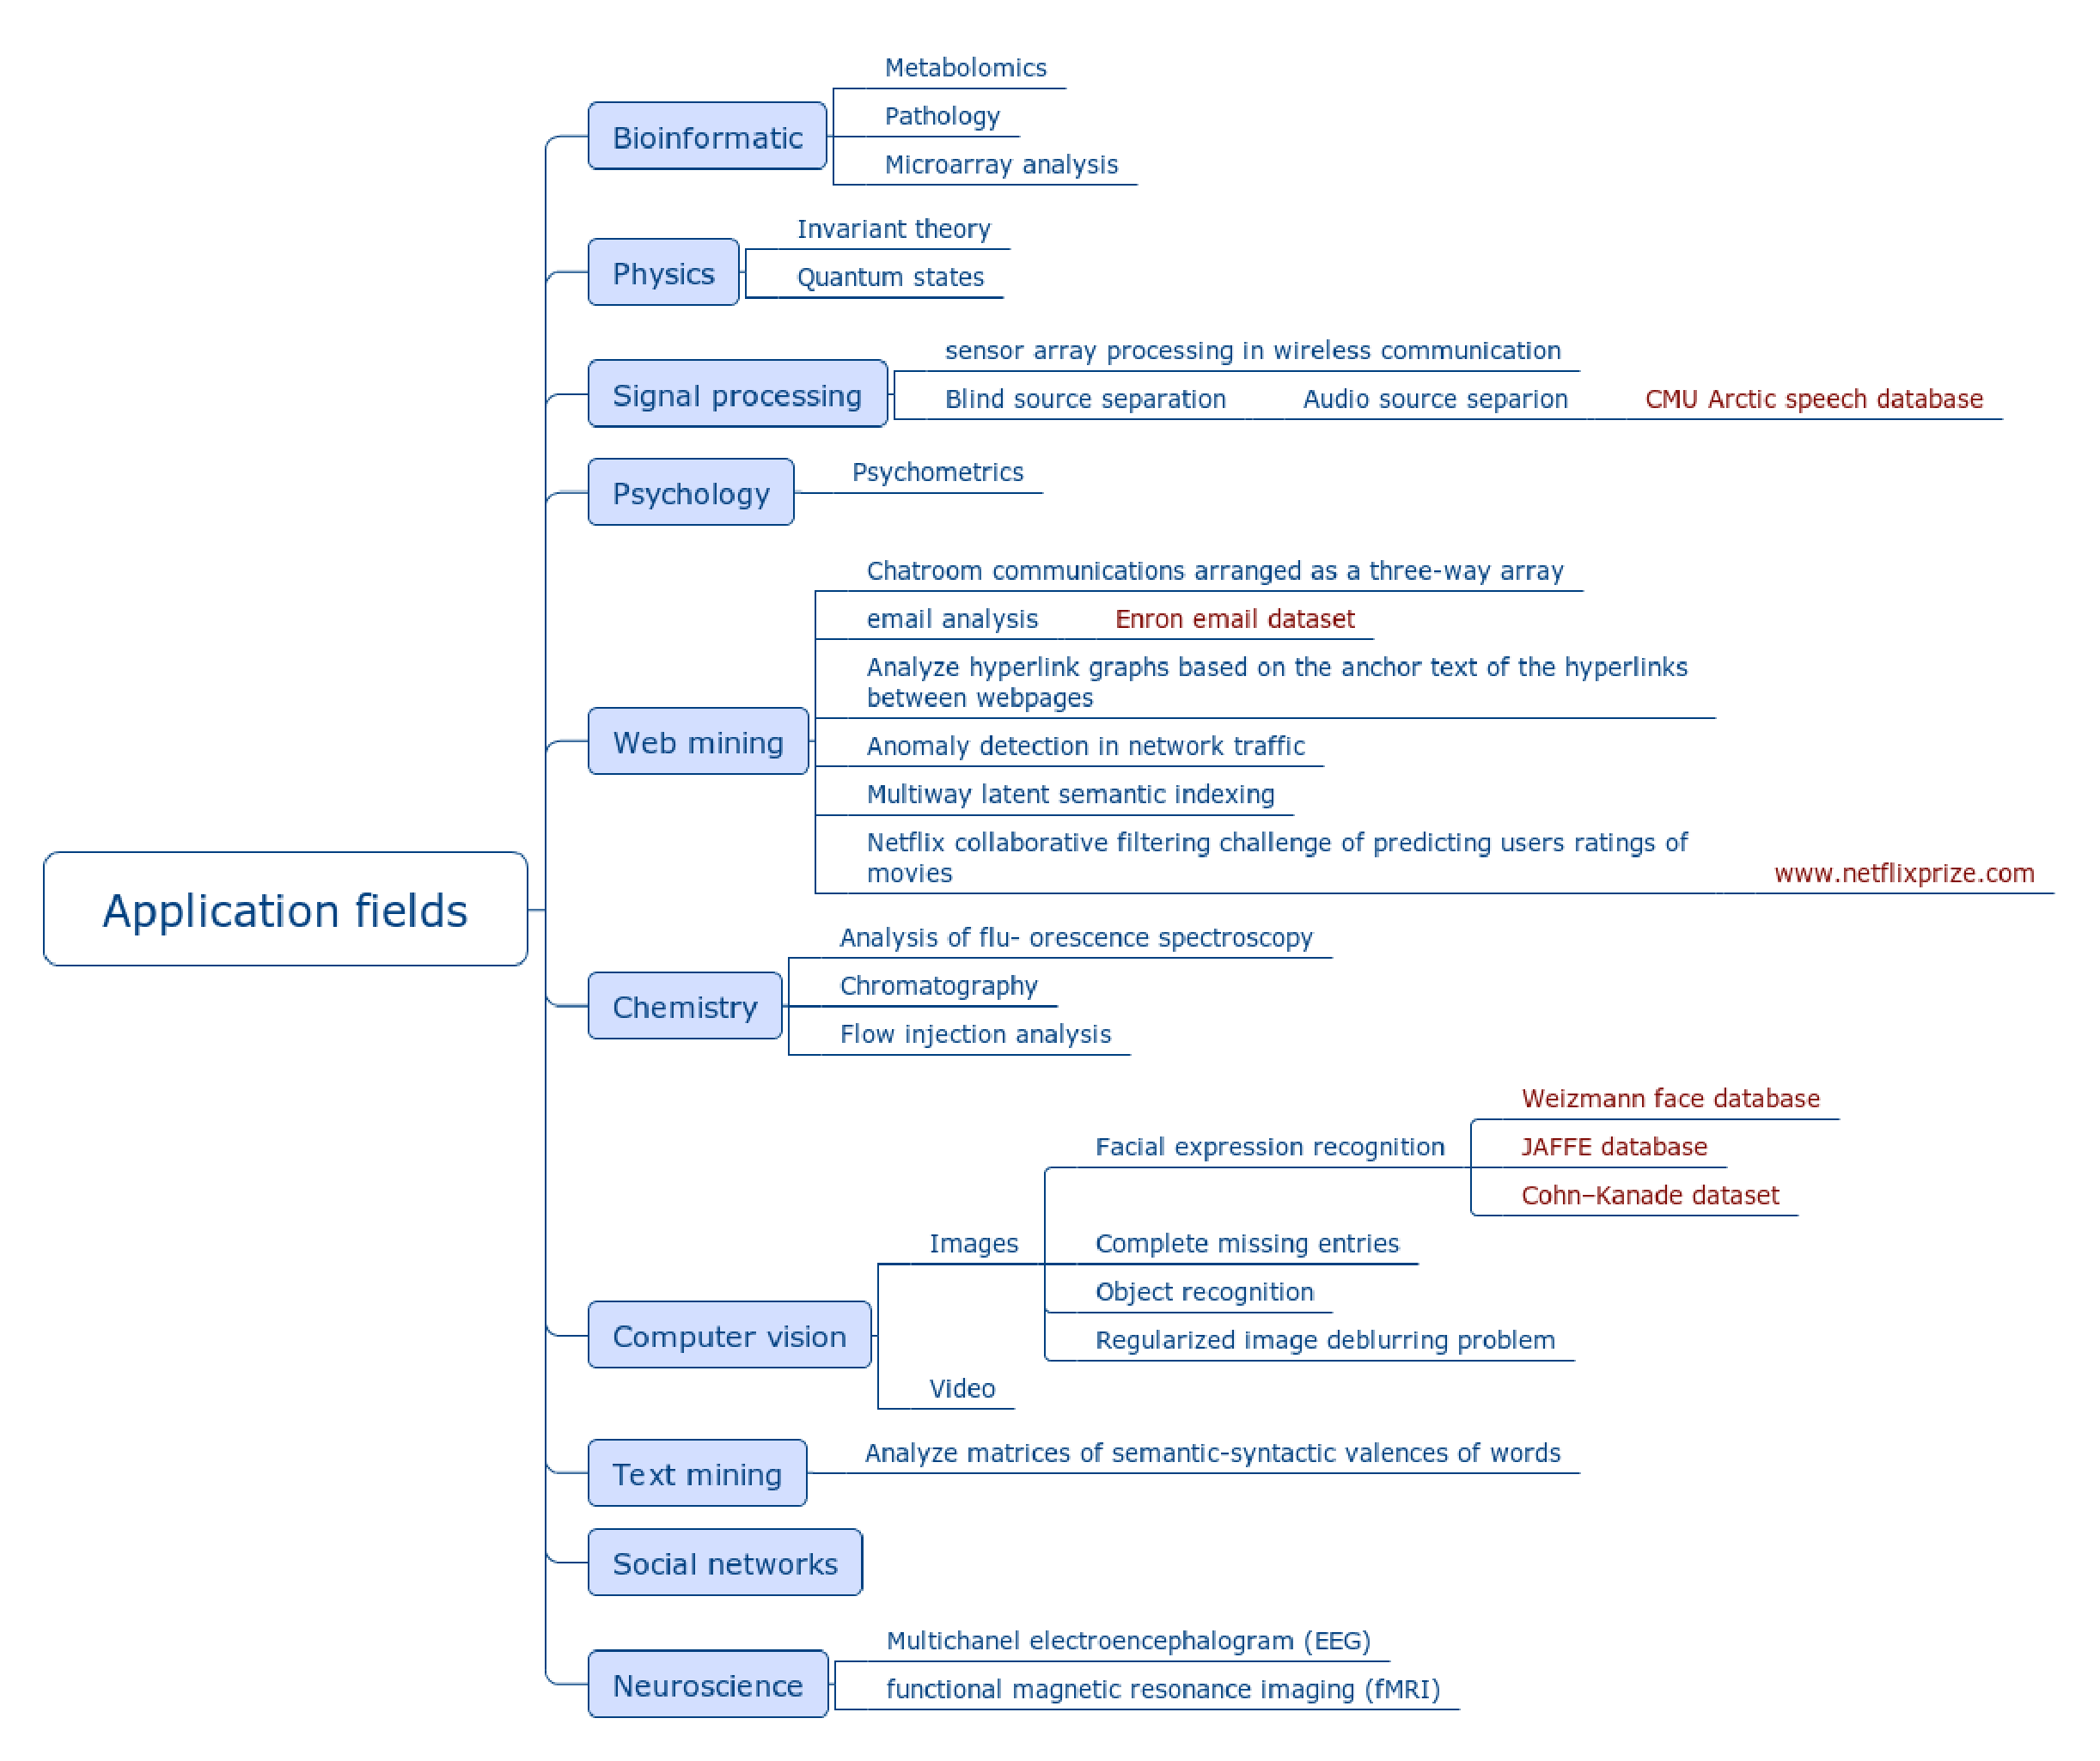
\includegraphics[scale=0.3]{Images/application_fields.eps}
 \caption{Application fields of tensor decomposition}\label{fig:applications}
\end{figure}


% Extend applications descriptions and cite paper and survey Specific for each field.


Fanaee and Gama \cite{Fanaee-T2016} introduce an interdisciplinary survey about tensor-based anomaly detection.


We suggest to readers to refer to Kolda \cite{Kolda2009}, Acar \cite{Acar2009} and \cite{Comon2014} for an exhaustive a detailed review of fundamental decomposition methods and applications. Furthermore, \cite{Dartois2016} presents tensor properties as extension of estructural properties of matrices.


\paragraph{Chemometrics}

\cite{Chaudhury2014} A computationally efficient technique for the solution of multi-dimensional PBMs of granulation via tensor decomposition

%bioinformatics
\paragraph{Bioinformatics}

In \cite{Acar2015} and \cite{Acar2014} a multimodal problem is addressed, the authors formulate data fusion as a coupled matrix and tensor factorization problem and discuss its extension to a structure-revealing data fusion model in metabolomics.


\paragraph{Image processing}

\cite{An2015} NNTF for facial expression recognition


\paragraph{Machine Learning}

\cite{Anandkumar2012} Tensor decompositions for learning latent variable models

\paragraph{Text mining}

\cite{Anisimov2014} This paper describes a method for automatic detection of semantic relations between concept nodes of a networked ontological knowledge base by analyzing matrices of semantic-syntactic valences of words. These matrices are obtained by means of nonnegative factorization of tensors of syntactic compatibility of words. 


\paragraph{Numerical analysis}
 
\cite{Antolin2015} use of the sum-factorization for the calculation of the integrals arising in Galerkin isogeometric analysis. While introducing very little change in an isogeometric code based on element-by-element quadrature and assembling, the sum-factorization approach, taking advantage of the tensor-product structure of splines or NURBS shape functions, significantly reduces the quadrature computational cost.

\cite{Benner2016} Fast iterative solution of the Bethe-Salpeter eigenvalue problem using low-rank and QTT tensor approximation.


\cite{Cherif2008} Blind identification of a second order Volterra-Hammerstein series using cumulant cubic tensor analysis.

\paragraph{Neuroscience}

\cite{Arnedo2015} Decomposition of brain diffusion imaging data uncovers latent schizophrenias with distinct patterns of white matter anisotropy, using NNTF to clustering.


\paragraph{Signal processing}

Cichocki et.al. \cite{Cichocki2015} sum up tensor decomposition approaches for signal processing problems.

Barker and Virtanen \cite{Barker2014} deal with monaural sound source separation problem using NNTF of modulation spectrograms.

\cite{Bilen2016} Necessity to manually assign the NTF components to audio sources in order to be able to enforce prior information on the sources during the estimation process, Automatic Allocation of NTF Components for User-Guided Audio Source Separation

\cite{Fitzgerald2006} propose a shifted 2D non-negative tensor factorisation algorithm which extends non-negative matrix factor 2D deconvolution to the multi-channel case. The use of this algorithm for multi-channel sound source separation of pitched instruments is demonstrated.

\paragraph{Other applications}

\cite{Espin-Noboa2016} Discovering and Characterizing Mobility Patterns in Urban Spaces: A Study of Manhattan Taxi Data. by using non-negative tensor factorization (NTF), we are able to cluster human behavior based on spatio-temporal dimensions. Second, for understanding these clusters, we propose to use HypTrails, a Bayesian approach for expressing and comparing hypotheses about human trails.

\cite{Figueiredo2014} NNTF factorization for household electrical seasonal consumption disaggregation



\begin{figure}[!ht]
\centering
 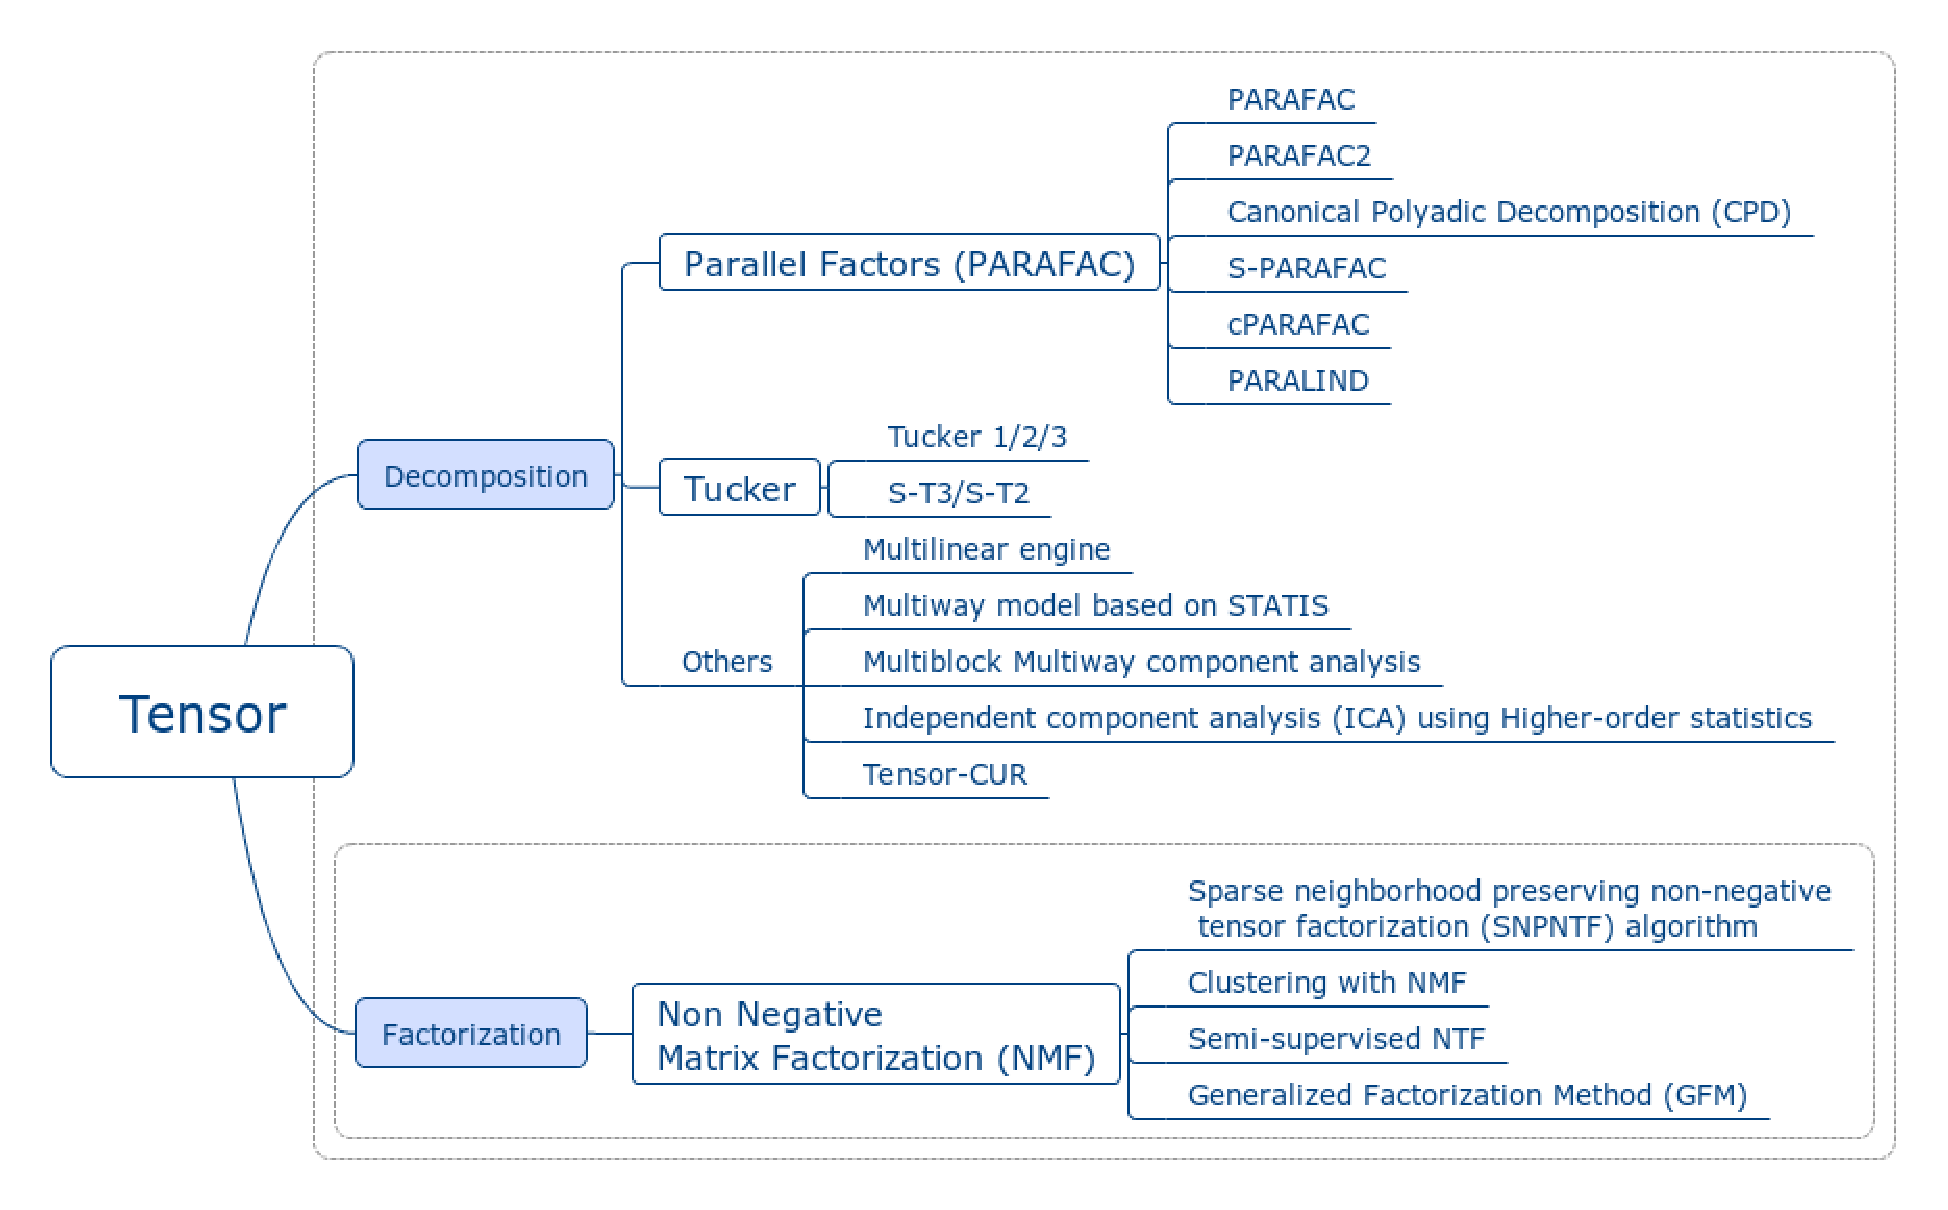
\includegraphics[scale=0.5]{Images/tensor_decomposition_methods.eps}\label{fig:methods}
 \caption{Tensor decomposition methods}
\end{figure}


\subsection{Canonica Polyadic Decomposition / PARAFAC}

Canonica Polyadic (CP) decomposition or PARAFAC decompose a tensor as a finite sum of rank-one tensors.

%figure

Domanov \cite{Domanov2015} shows relaxed uniqueness conditions and algebraic algorithm for Canonical polyadic decomposition, as well as a reduction to generalized eigenvalue decomposition \cite{Domanov2014} and uniqueness properties \cite{Domanov2013} of third-order tensors.


% \subsection{TUCKER Decomposition}




\subsection{Other methods}

\cite{Bernardi2013} The tensor decomposition addressed in this paper may be seen as a generalization of Singular Value Decomposition of matrices. We consider general multilinear and multihomogeneous tensors. We show how to reduce the problem to a truncated moment matrix problem and give a new criterion for flat extension of Quasi-Hankel matrices. We connect this criterion to the commutation characterization of border bases.


\subsection{Tensor completion}

Acar et.al \cite{Acar2011} presents a scalable tensor factorization method to deal with completion problem using PARAFAC method.

\cite{Cao2015} The existing studies involving matrix or tensor completion problems are commonly under the nuclear norm penalization framework due to the computational efficiency of the resulting convex optimization problem. Folded-concave penalization methods have demonstrated surprising developments in sparse learning problems due to their nice practical and theoretical properties. To share the same light of folded-concave penalization methods, we propose a new tensor completion model via folded-concave penalty for estimating missing values in tensor data. Two typical folded-concave penalties, the minmax concave plus (MCP) penalty and the smoothly clipped absolute deviation (SCAD) penalty, are employed in the new model. To solve the resulting nonconvex optimization problem, we develop a local linear approximation augmented Lagrange multiplier (LLA-ALM) algorithm which combines a two-step LLA strategy to search a local optimum of the proposed model efficiently. Finally, we provide numerical experiments with phase transitions, synthetic data sets, real image and video data sets to exhibit the superiority of the proposed model over the nuclear norm penalization method in terms of the accuracy and robustness.

\cite{Chen2014} The success of research on matrix completion is evident in a variety of real-world applications. Tensor completion, which is a high-order extension of matrix completion, has also generated a great deal of research interest in recent years. Given a tensor with incomplete entries, existing methods use either factorization or completion schemes to recover the missing parts. However, as the number of missing entries increases, factorization schemes may overfit the model because of incorrectly predefined ranks, while completion schemes may fail to interpret the model factors. In this paper, we introduce a novel concept: complete the missing entries and simultaneously capture the underlying model structure. To this end, we propose a method called simultaneous tensor decomposition and completion (STDC) that combines a rank minimization technique with Tucker model decomposition. Moreover, as the model structure is implicitly included in the Tucker model, we use factor priors, which are usually known a priori in real-world tensor objects, to characterize the underlying joint-manifold drawn from the model factors. By exploiting this auxiliary information, our method leverages two classic schemes and accurately estimates the model factors and missing entries. We conducted experiments to empirically verify the convergence of our algorithm on synthetic data and evaluate its effectiveness on various kinds of real-world data. The results demonstrate the efficacy of the proposed method and its potential usage in tensor-based applications. It also outperforms state-of-the-art methods on multilinear model analysis and visual data completion tasks.

Following Ji Lu et.al \cite{Liu2013} notation

low rank matrix completion

\begin{equation} 
 \begin{split}
  \min_X & \text{ rank}(X)\\
  \text{s.t. } & X_\Omega = M_\Omega
 \end{split}
\end{equation}
where $\Omega$ is an index set, then $X_\Omega$ is coping entries of $X$ in the 
indexes $\Omega$ and missed entries $\hat{\Omega}$ would be $0$

The missing entries in $X$ are determined in order to minimize the matrix $X$ 
rank. i.e. a non convex optimization problem since rank is nonconvex.

Frequently, trace norm (or nuclear norm) $||\cdot ||_*$ is used to approximate 
the rank of matrices.
Trace norm is the tighest convex envelop for the matrices rank.

\begin{equation} 
 \begin{split}
  \min_X & ||X||_*\\
  \text{s.t. } & X_\Omega = M_\Omega
 \end{split}
\end{equation}

Since tensor is a generalization of the matrix concept, we generalize the 
optimization problem as

\begin{equation} 
 \begin{split}
  \min_{\mathcal{X}} & ||\mathcal{X}||_*\\
  \text{s.t. } & \mathcal{X}_\Omega = \mathcal{T}_\Omega
 \end{split}
\end{equation}

Where $\mathcal{X}$ and $\mathcal{T}$ are $n$-order tensors with identical size.



% \subsection{Tensor probability}

% Given a sample set


\subsection{Kernel methods}

In contrast with traditional learning techniques, kernel methods do not need a vectorial representation of data. Instead, they use a kernel function. Therefore, kernel methods are naturally applied to unstructured, or complex structured, data such as texts, strings, trees and images \cite{shawe2004kernel}. 

Informally, a kernel function measures the similarity of two objects. Formally, a kernel function, $k:X\times X\rightarrow\mathbb{R}$,
maps pairs $(x,y)$ of objects in a set $X$, the problem space, to the reals. A kernel function implicitly generates a map, $\Phi:X\rightarrow F$, where $F$ corresponds to a Hilbert space called the feature space. The dot product in $F$ is calculated by $k$, specifically $k(x,y)=<\Phi(x),\Phi(y)>_{F}$. Given an appropriate kernel function, complex patterns in the problem space may correspond to simpler patterns in the feature space. For instance, non-linear patterns in the problem space may correspond to linear patterns in the feature space. 

Both $k$-means and SNMF have kernelized versions, which receive as input a kernel matrix instead of a set of sample represented by feature vectors. The kernel version of $k$-means is called, unsurprisingly, kernel $k$-means (KKM). In the case of SNMF, the kernelized version works as follows.

SNMF starts with an initial estimation of the matrix factor $H$ and iteratively update it using the updating equation:

\[
H_{i,k}=H_{i,k}(1-\beta+\beta\frac{((X^{T}X)H)_{i,k}}{(HH^{T}H)_{i,k}})
\]


The kernel version of the algorithm is obtained by using a kernel matrix $K$ instead of the expression $(X^{T}X)$, where $K$ is an
$l\times l$ matrix with $K_{i,j}=k(x_{i},x_{j}).$ There are different types of kernels some of them general and some of them specifically defined for different types of data. The most popular general kernels are the linear kernel 

\begin{equation}
k(x,y)=<x,y>,\label{eq:id-kernel}
\end{equation}

 the polynomial kernel 
 
\[
k(x,y)=p(<x,y>),
\]

 where $p(\,)$ is a polynomial with positive coefficients, and the Gaussian (or RBF) kernel 
 
\begin{equation}
k(x,y)=e^{\frac{\left\Vert x-y\right\Vert ^{2}}{2\sigma^{2}}}.\label{eq:Gaussian-kernel}
\end{equation}


The cluster centroids estimated by the kernel versions of both algorithms are in the feature space and correspond to the points $C_{j}=\frac{1}{n}\sum_{x_{i}\in C_{j}}\Phi(x_{i})$. However, we are interested on the pre-image in the original space of this centroids, i.e., points $\hat{C}_{j}$ such that $\Phi(\hat{C}_{j})=C_{j}$. However, it is possible that a exact pre-image may not even exist, so we look for the $\hat{C}_{j}$ that minimizes the following objective function:$\min_{\hat{C}_{j}}\left\Vert \hat{C}_{j}-C_{j}\right\Vert ^{2}$. According to Kwok et al. \cite{kwok2004preimage}, the optimum $C_{j}$ can be found by iterating the following fixed-point formula:

\begin{equation}
\hat{C}_{j}^{t+1}=\frac{\sum_{i=1}^{N}\exp(\frac{-||\hat{C}_{j}^{t}-x_{i}||)}{s})x_{i}}{\sum_{i=1}^{N}\exp(\frac{-||\hat{C}_{j}^{t}-x_{i}||}{s})}\label{eq:back-projection}
\end{equation}


\section{Kernel Non-negative Matrix Factorization}

Kernel Non-negative Matrix Factorization (KNMF) can be naturally derivated of convex NMF (insert cites 92, 98 and 120 from Cichocki book). Given a kernel function $\phi:x\in X \rightarrow \phi(x)\in F $, mapping for $N$ elements $\phi(X) = [ \phi(x_1),\ldots \phi(x_N) ]$. Then, KNMF can be defined as
\begin{equation}
 \phi(X)\cong\phi(X)WH^T
\end{equation}\label{eq:KNMF}

Therefore, the cost function to minimize is

\begin{equation}
 || \phi(X) - \phi(X)WH^T ||_F^2 = tr(K) - 2 tr(H^TKW)+tr(W^TKWH^TH)
\end{equation}

 Where kernel $K=\phi^T(X)phi(X)$


\section{Problem Statement}

The general problem addressed by this research proposal is the design of non-supervised learning algorithms, in particular tensor factorization algorithms, applied in the space induced by a kernel function. Matrix and analogous tensor factorization is central to different important tasks in machine learning and information retrieval such as: clustering, latent topic analysis, recommendation, among others. Another important focus of this research is to study robustness from a kernel method perspective. 

Kernel methods are ubiquitous in machine learning and there are some connections between some types of kernels (Guassian kernels) and robustness that has not been fully explored yet. The general research question to be addressed by this research is whether the use of some types of kernels may bring robustness to particular factorization methods. A satisfactory solution of this general challenge requires to answer some particular \textbf{research question}: 

\begin{itemize}
 \item How to decompose tensors in an space induced by a kernel function? %- exploratory
\end{itemize}

An answer to the question derivate in a method which factorize a given tensor in the feature space induced by a Kernel function. Naturally, to inquire about the effects of decompose tensors in an space induced by a kernel function open space to evaluate the proposal method performance as well as its capabilities dealing with multimodal data, scalability and robustness to noise and outliers.




%  \item \textbf{GENERAL AND SPECIFIC OBJECTIVES} 
% 7. OBJETIVO GENERAL Y OBJETIVOS ESPECÍFICOS: (Evaluables)

% \subsection*{General objective}
% 
% 
% 
% \subsection*{Specific objectives}
% 
% \item \textbf{METHODOLOGY}\\ 
% % 8. METODOLOGÍA: (Descripción del procedimiento a emplear para obtener los 
% objetivos propuestos).
% % 
% 
% \end{enumerate}
% 
% %  \item \textbf{ACTIVITIES} \\
% % 9. ACTIVIDADES A DESARROLLAR:
% 
% 
% Project activities and results are structured within \textit{Work Packages} 
% (WP) in terms of \textit{Tasks} and \textit{Deliverables}, as described below.
% 
% \subsection*{WP0: PROPOSSAL}
% 
% This WP will assure a suitable scope of propossal due to evaluation of risk 
% and feasibility. In addition, activities and schedule will be delimited in 
% concordance with objectives stablished.
% 
% \subsubsection*{TASKS}
% \begin{itemize}
%  \item T0.1: Propossal review
%  \item T0.2: Literature review.
% \end{itemize}
% 
% 
% \subsubsection*{DELIVERABLES}
% \begin{itemize}
%  \item D0.1: A survey paper reporting the literature review.
%  \item D0.2: Final propossal
% \end{itemize}
% 
% 
% \subsection*{WP1: MANAGEMENT }
% 
% This WP will ensure effective planning, implementation, coordination and achievement of the project activities, including successful completion of the tasks and timely production of deliverables.
% 
% \subsubsection*{TASKS }
% \begin{itemize}
% \item T1.1: ADMINISTRATION AND MANAGEMENT. Will take care of financial and resource accounting. It will also be in charge of managing the relations with collaborating institutions and administrative bodies within.
% \item T1.2: PROJECT FOLLOW UP AND QUALITY CONTROL. Will act as the final stage before delivery hand over to ensure compliance and coherence. Also, it will follow up project progress anticipating corrective actions and assessing risk mitigation actions.
% \end{itemize}
% 
% \subsubsection*{DELIVERABLES}
% \begin{itemize}
% \item D1.1: Periodic technical project reports.
% % \item D1.2: Periodic financial project reports
% \end{itemize}
% 
% \subsection*{WP2: MEASURING ROBUSTNESS}
% 
% 
% \subsubsection*{TASKS }
% 
% \subsubsection*{DELIVERABLES }
% 
% \subsection*{WP3: DESIGN OF ROBUST MATRIX FACTORIZATION ALGORITHMS}
% 
% \subsubsection*{TASKS }
% 
% \subsubsection*{DELIVERABLES }
% 
% \subsection*{WP4: PERFORMANCE EVALUATION}
% 
% 
% \subsubsection*{TASKS }
% 
% \subsubsection*{DELIVERABLES }
% 
% \subsection*{WP5: DISSERTATION}
% \subsubsection*{TASKS}
% \subsubsection*{DELIVERABLES }
% 
% \clearpage
% 
% %  \item \textbf{SCHEDULE}\\
% % 10. CRONOGRAMA:
% 
% 
% %  \item \textbf{BIBLIOGRAPHY:}\\
% % 11. BIBLIOGRAFÍA BÁSICA:
% 
\begin{thebibliography}{References}

\bibliographystyle{plain}
 \bibliography{refs} 
 
\end{thebibliography}
% 
% 
% %  \item \textbf{EQUIPMENT AND SUPPLIES}\\
% % 12. RECURSOS FÍSICOS: (Especificar la disponibilidad y adjuntar carta de 
% compromiso de la dependencia o empresa cuando sea necesario).
% A work station with a computer with internet and bibliographic material.
% 
% 
% %  \item \textbf{COSTS AND FINANCIAL SOURCES}\\
% % 13. COSTOS DEL TRABAJO Y FUENTES DE FINANCIACIÓN:
% 
% \begin{table}[!h]
% \centering
% \begin{tabular}{l l r}
% \hline
%  \textbf{Concept} & \textbf{Source} & \textbf{Total cost}* \\
%  \hline
%  Salary researcher & Researcher & \$144 \\
%  Advisor salary & Universidad Nacional de Colombia & \$80\\
%  Conferences and events & Universidad Nacional de Colombia/Researcher & \$10 
% \\
%  \hline
%  Notebook & Researcher & \$2\\
%  Desktop computer & Research group MindLAB & \$1.6\\
%  High performance computer & Research group MindLAB & \$20\\
%  \hline
%  Office supplies & Researcher & \$1.5\\
%  Bibliography & Universidad Nacional de Colombia & \$1\\
%  \hline
%  \textbf{Total} & & \textbf{\$260.1}
% \end{tabular} 
% \end{table}
% \textit{*Millions of colombian pesos (COP)}
% 
% 
% 
% 
% %  \item COMMENTARY WITH ADVISOR APROVAL
% % 14. COMENTARIO CON VISTO BUENO DEL DIRECTOR: (calificar los siguientes 
% aspectos: organización, pertinencia, relevancia y originalidad).
% %  \item BIDDER SIGNATURE 
%  
%  Robinson Andr\'es Jaque Pirab\'an
% % 15. FIRMA DEL PROPONENTE
% %  \item SIGNATURE OF ADVISOR
% % 16. FIRMA DEL DIRECTOR (ASESORES)
% % 17. FECHA
%  
% % \end{enumerate}
% 
% 
% 
% 
\end{document}
